\documentclass[border=15pt, multi, tikz]{standalone}
\usepackage{import}
\usepackage{scalefnt}
\subimport{./layers/}{init}
\usetikzlibrary{positioning}
\usetikzlibrary{decorations.pathreplacing,calligraphy}

\def\ConvColor{rgb:yellow,5;red,2.5;white,5}
\def\ConvReluColor{rgb:yellow,5;red,5;white,5}
\def\PoolColor{rgb:red,1;black,0.3}
\def\DcnvColor{rgb:blue,5;green,2.5;white,5}
\def\SoftmaxColor{rgb:magenta,5;black,7}
\def\SumColor{rgb:blue,5;green,15}
\def\poolsep{0.5}


\begin{document}

\makeatletter

\tikzset{
    dot diameter/.store in=\dot@diameter,
    dot diameter=3pt,
    dot spacing/.store in=\dot@spacing,
    dot spacing=10pt,
    dots/.style={
        line width=\dot@diameter,
        line cap=round,
        dash pattern=on 0pt off \dot@spacing
    }
}
\makeatother
\scalefont{0.7}
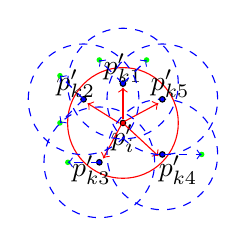
\begin{tikzpicture}
\tikzstyle{connection}=[ultra thick,every node/.style={sloped,allow upside down},draw=\edgecolor,opacity=0.6]
%%%%%%%%%%%%%%%%%%%%%%%%%%%%%%%%%%%%%%%%%%%%%%%%%%%%%%%%%%%%%%%%%%%%%%%%%%%%%%%%%%%%%%%%
%% Draw Layer Blocks
%%%%%%%%%%%%%%%%%%%%%%%%%%%%%%%%%%%%%%%%%%%%%%%%%%%%%%%%%%%%%%%%%%%%%%%%%%%%%%%%%%%%%%%%
% core point
\draw[color=red](2.5,1.5) circle (20pt);
\fill[color=red] (2.5,1.5) circle (1pt);
\draw[color=black,thin](2.5,1.5) circle (1pt);
\node[shift={(2.5,1.3)},align=center] {$p'_i$};
\draw[->,color=red] (2.5,1.55) --(2.5,1.95);
\draw[->,color=red] (2.45,1.5) --(2.05,1.75);
\draw[->,color=red] (2.48,1.48) --(2.25,1.05);
\draw[->,color=red] (2.52,1.48) --(2.95,1.08);
\draw[->,color=red] (2.52,1.52) --(2.95,1.75);

\draw[color=blue,dashed](2.5,2) circle (20pt);
\fill[color=blue] (2.5,2) circle (1pt);
\draw[color=black,thin](2.5,2) circle (1pt);
\node[shift={(2.5,2.2)},align=center] {$p'_{k1}$};

\fill[color=green] (2.2,2.3) circle (1pt);
\draw[->,color=blue,dashed] (2.5,2) --(2.2,2.3);
\fill[color=green] (2.8,2.3) circle (1pt);
\draw[->,color=blue,dashed] (2.5,2) --(2.8,2.3);

\draw[color=blue,dashed](2,1.8) circle (20pt);
\fill[color=blue] (2,1.8) circle (1pt);
\draw[color=black,thin](2,1.8) circle (1pt);
\node[shift={(1.9,2)},align=center] {$p'_{k2}$};

\fill[color=green] (1.7,2.1) circle (1pt);
\draw[->,color=blue,dashed] (2,1.8) --(1.7,2.1);
\fill[color=green] (1.7,1.5) circle (1pt);
\draw[->,color=blue,dashed] (2,1.8) --(1.7,1.5);

\draw[color=blue,dashed] (2.2,1) circle (20pt);
\fill[color=blue] (2.2,1) circle (1pt);
\draw[color=black,thin](2.2,1) circle (1pt);
\node[shift={(2.1,0.9)},align=center] {$p'_{k3}$};

\fill[color=green] (1.8,1) circle (1pt);
\draw[->,color=blue,dashed] (2.2,1) --(1.8,1);

\draw[color=blue,dashed] (3,1.1) circle (20pt);
\fill[color=blue] (3,1.1) circle (1pt);
\draw[color=black,thin](3,1.1) circle (1pt);
\node[shift={(3.2,0.9)},align=center] {$p'_{k4}$};
\fill[color=green] (3.5,1.1) circle (1pt);
\draw[->,color=blue,dashed] (3,1.1) --(3.5,1.1);

\draw[color=blue,dashed] (3,1.8) circle (20pt);
\fill[color=blue] (3,1.8) circle (1pt);
\draw[color=black,thin](3,1.8) circle (1pt);
\node[shift={(3.1,2)},align=center] {$p'_{k5}$};
%%%%%%%%%%%%%%%%%%%%%%%%%%%%%%%%%%%%%%%%%%%%%%%%%%%%%%%%%%%%%%%%%%%%%%%%%%%%%%%%%%%%%%%%

%%%%%%%%%%%%%%%%%%%%%%%%%%%%%%%%%%%%%%%%%%%%%%%%%%%%%%%%%%%%%%%%%%%%%%%%%%%%%%%%%%%%%%%%
%%% Draw connections
%%%%%%%%%%%%%%%%%%%%%%%%%%%%%%%%%%%%%%%%%%%%%%%%%%%%%%%%%%%%%%%%%%%%%%%%%%%%%%%%%%%%%%%%
% \draw[connection] (0,0,0) --node{}++(0,0,15) --node{}++(5,0,0) --node{}++(0,0,-15) --node{}++(-5,0,0);
% \draw[connection] (0,3,0) --node{}++(0,0,15) --node{}++(5,0,0) --node{}++(0,0,-15) --node{}++(-5,0,0);
% \draw[connection] (0,0,0) --node{}++(0,3,0);
% \draw[connection] (5,0,15) --node{}++(0,3,0);
% \draw[connection] (5,0,0) --node{}++(0,3,0);
% \draw[connection] (0,0,15) --node{}++(0,3,0);
%%%%%%%%%%%%%%%%%%%%%%%%%%%%%%%%%%%%%%%%%%%%%%%%%%%%%%%%%%%%%%%%%%%%%%%%%%%%%%%%%%%%%%%%

\end{tikzpicture}
\end{document}\grid